\documentclass[letterpaper,10pt,serif,draftclsnofoot,onecolumn,compsoc,titlepage]{IEEEtran}

\usepackage{graphicx}                                        
\usepackage{amssymb}                                         
\usepackage{amsmath}                                         
\usepackage{amsthm}                                          
\usepackage{cite}
\usepackage{alltt}                                           
\usepackage{float}
\usepackage{color}
\usepackage{url}
\usepackage{pgfgantt}
\usepackage{rotating}

\usepackage{balance}
\usepackage[TABBOTCAP, tight]{subfigure}
\usepackage{enumitem}

\usepackage{geometry}
\geometry{margin=.75in}
\usepackage{hyperref}
%\usetikzlibrary{shapes, positioning, calc}
\usepackage{caption}
\usepackage{listings}
%\usepackage[utf8]{inputenc}
%pull in the necessary preamble matter for pygments output

%% The following metadata will show up in the PDF properties
\hypersetup{
   colorlinks = true,
   citecolor = black,
   linkcolor = black,
   urlcolor = black,
   pdfauthor = {Shu-Ping Chien, Brock Smedley, and W Keith Striby Jr},
   pdfkeywords = {CS461 "Senior Project" Requirements Document},
   pdftitle = {CS 461 Requirements Document},
   pdfsubject = {CS 461 Requirements Document},
   pdfpagemode = UseNone
}

\parindent = 0.0 in
\parskip = 0.1 in
\title{Requirements Document: Multi-Camera, System-on-Chip (SoC) Based, Real-Time Video Processing for UAS and VR/AR Applications}
\author{Group 51: Shu-Ping Chien, Brock Smedley, and W Keith Stirby Jr \\ 03 November 2017 \\ CS-461, Senior Software Engineering Project, Fall 2017}
\begin{document}
\begin{titlepage}
\maketitle
\begin{abstract}

WRITE ME \\

\end{abstract}
\end{titlepage}
\newpage

\tableofcontents
\newpage

\section{Introduction}

\subsection{Purpose}

This software requirements specification is intended to define the requirements of the 
project of developing a multi-camera, multispectral image processing system, that 
operates on a System-on-Chip (SoC) at near-real-time, for use in ground and air based 
applications. Defined requirements will allow for a contract between us, the 
developers, and Rockwell Collins, our client, on what Rockwell Collins wants us to 
deliver in their desired software. This document is intended for review and reference 
by both the developers and the clients.\\

\subsection{Scope}

The product outlined in this requirements document will be the multi-camera, SoC based,
 real-time video processing for UAS and VR/AR applications. This product will need to 
 be able to generate a stitched video output from a multi-camera input. The product is 
 intended to help initialize our client's development of a cheaper alternative to a 
 product that is already offered to their customers.\\

The software products that will be produced include software for a stitched video output 
from the NVIDIA Jetson TX1 or TX2, receiving the input from two visible band cameras. 
The video output is expected to be near-real-time, and the latency from the camera 
input to the video output is expected to be improved upon throughout the project. Video 
output stretch goals is to have software that fuses the video output from the input of 
three, four, five, and six cameras, and have up to four infrared band inputs.\\

Output display stretch goals will be to incorporate inertial measurement unit (IMU) 
data, orientation tracking data, GPS data, and geolocate imagery. Two final stretch 
goals are packaging the hardware for flight, and interfacing the system to support
the client's desired cameras for flight use.\\

The goal of the software is to contribute to a project that will assist pilots during 
low visibility conditions during the day, night, and inclement weather for all phases 
of flight. The video input from infrared and visible band cameras combined with 
on-board sensor input, and databases will enhance a pilot vision for an unmanned and 
manned aerial vehicle.\\

\subsection{Definitions, Acronyms, Abbreviations}

...

\subsubsection{Definitions}

multiple cameras - at least two cameras, but a maximum of six cameras for video input.

\subsubsection{Acronyms}

MAKE THIS INTO A TABLE\\
Term
Acronym\\
CSI
Camera Serial Interface\\
EVS
Enhanced Vision System\\
GPU
Graphic Processing Unit\\
ISP
Image Signal Processors\\
HUD
Head-up Display\\
SoC
System on a chip\\
SOM
System on a module\\
SWaP-C
Size, weight, power and cost\\
VI
Video Input\\
UAV
Unmanned Aerial Vehicle\\

\subsubsection{Abbreviations}

...

\subsection{References}

...

\subsection{Overview}

This project aims to create a device that is capable of combining the video input from 
two or more cameras and produce and output at near-real time. Our proposed solution 
will use an NVIDIA Jetson device, which we will use for its integrated GPU.\\

We need this GPU to combine the images from multiple cameras. The end goal is to have 
a system that uses the input from multiple cameras that operate on different bands of 
the electromagnetic spectrum; infrared, ultraviolet, and visible light, among others. 
 By using these varying bands, we should be able to produce an image that can be used 
 to see in low-visibility situations, such as landing a UAV in fog.\\

The images we produce will be 2D representations of our collective image captures. In 
other words, we do not aim to create a 3D image or a dynamic focus image. This is 
certainly possible when using multiple cameras, but we simply aim to use multiple 
cameras on different spectral bands to create one image of one subject that is the 
combination of all images captured by the cameras.\\


\section{Overall Description}

\subsection{Product Perspective}

The system will be self-contained and consists of three parts: one NVIDIA TX1 or 2 board, 
one CSI carrier board, and at least two cameras. The cameras connect to the CSI board, 
which is connected to the NVIDIA board. The NVIDIA board is responsible for decoding 
the serial data retrieved by the CSI board from the cameras, and is then be used to 
execute the software for image processing and combining images from multiple cameras.\\

\begin{figure}[H]
	\centering
	\label{fig:CopyOnWriteBefore}
	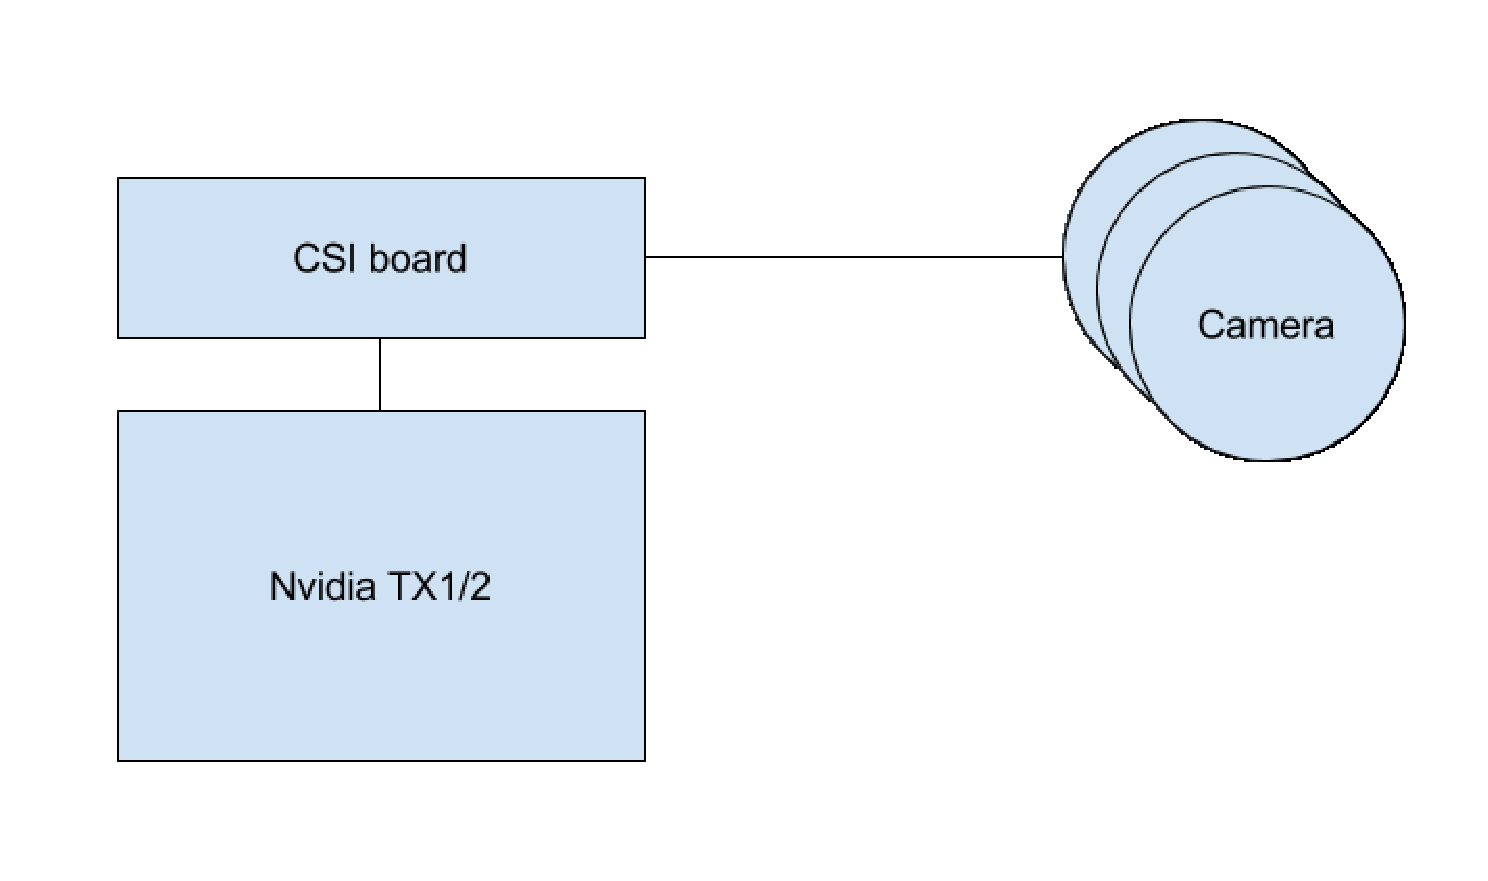
\includegraphics[width=8cm,height=3.25cm]{images/block_diagram.eps}
	\caption{Product Block Diagram \label{overflow}}
\end{figure}

\subsection{Production Functions}

The EVS will be able to capture images from different spectral bands to create the 
clearest possible image in situations where visible light does not provide enough 
clarity. These images will be relayed in near-real time so that it can be used as a 
video feed. One use case would be for a pilot to be able to see the ground when landing 
in low-visibility conditions.\\

Since the EVS will be able to provide near to all weather operations, the images from 
the system will be analyzed and combined in several modes. The mode of equivalent 
vision can display images shot by cameras directly in normal visibilities condition 
such as clear daytime. The mode of synthetic vision will display images from the 
channels provide thermal images of the landscape and various types of lighting, for 
example incandescent, halogen, and LED lights, etcetera. Then the view on the display 
device will be real images combined with light structure.\\

\subsection{Constraints}

The system must operate in near-real time. In other words, the camera feed(s) must be 
processed quickly enough for the user to make snap decisions based on the feed. The 
NVIDIA board should process each frame before the next one arrives to be processed. 
If we’re recording at 30 frames per second (fps), then each output frame should be 
processed in less than 1/30 of a second.\\

\subsection{Assumptions \& Dependencies}

LIST ITEMS, WRONG, THIS SHOULD BE IN PARAGRAPH FORM\\
Software deployed on NVIDIA TX1/2 with NVIDIA Jetpack from Ubuntu machine
Adequate power supplies being used
Cameras being aimed at same subject; capturing mostly the same image
Each camera works independently of the system

\section{Specific Requirements}
THIS NEEDS TO BE IN PARAGRAPH FORM, WITH SECTIONS FROM THE IEEE STD 830-1998\\

\subsection{TX1/2}
		\subitem Adequate power supply
		\subitem NVIDIA Jetpack software + Ubuntu system to deploy it\\
\subsection{CSI Board}
		Camera serial interface is the hardware that interfaces with different cameras or image sensors, which provides output for a computer with pixel data and signals that can be used for subsequent image processing. Therefore, the CSI is the way to be used to transfer camera input to computer in this project.
		In order to carry up to six cameras, a carrier board with CSI such as J106 is required to connect cameras and NVIDIA TX1/2, and the video output format from CSI is depending on different chosen cameras.\\

\subsection{Cameras}
		\subitem Visible light
		\subitem Infrared
		\subitem UV
		\subitem ...\\

\newpage
	\section{Development Schedule}

	%See gantt chart, figure 2 on page 7.\\
	%still in under construction\\
	%\begin{figure}
	%\centering
	%\begin{tikzpicture}
	%\begin{pgfinterruptboundingbox}
	\begin{rotate}{270}
	%\section{Development Schedule}
    \begin{ganttchart}
    	[x unit=1.0mm, time slot format=isodate]
    	{2017-11-01}{2018-05-31}
    	\gantttitlecalendar{year, month=name}\\
    	\ganttbar{Task 1}{2017-11-01}{2017-11-30}\\
    	\ganttbar{Task 2}{2017-11-15}{2018-01-06}\\
    	\ganttbar{Task 3}{2018-01-01}{2018-01-31}\\
    	\ganttbar{Task 4}{2018-01-15}{2018-02-28}\\
    	\ganttbar{Task 5}{2018-03-01}{2018-03-31}\\
    	\ganttbar{Task 6}{2018-04-01}{2018-04-30}\\
    	\ganttbar{Task 7}{2018-05-01}{2018-05-31}\\
    \end{ganttchart}
    \newline
    \newline
    \newline
    \newline
    \newline
    \newline
    \newline
    \newline
	Fig. 2: Project Schedule
	\newline
	%\endcentering
    \end{rotate}
    %\end{pgfinterruptboundingbox}
%\useasboundingbox (frame.south west) rectangle (frame.north east);    
%\end{tikzpicture}
%\caption Fig. 2: Project Schedule
%\end{figure}
\newpage	
\newpage
\newpage
	

\subsection{Development Schedule Tasks}
Task 1: Have hardware procured and assembled.\\
Task 2: Produce a tiled video output from the input of six cameras.\\
Task 3: Produce stitched video output from the input of two and three cameras, 
and have latency estimates produced.\\
Task 4: Produce a dual stitched video output that is combined into a fused 
five-camera output (stretch goal).\\
Task 5: Incorporate IMU data, orientation tracking data, GPS data, and 
geolocate imagery into the video output (stretch goals).\\
Task 6: Package the system hardware for flight (stretch goal).\\
Task 7: Produce a software interface for the system to accomodate higher 
quality cameras (stretch goal).\\

%\newpage



\end{document}
